\question[20] A loop of wire with radius $R=15$ cm lies as shown in a region where there is a uniform magnetic field coming out of the page. The magnetic field is changing with time:
\begin{equation*}
	B(t)=B_0 e^{-\frac{t}{\tau}}
\end{equation*}
Where $B_0=0.5$ T and $\tau=0.02$ s.

\begin{center}
	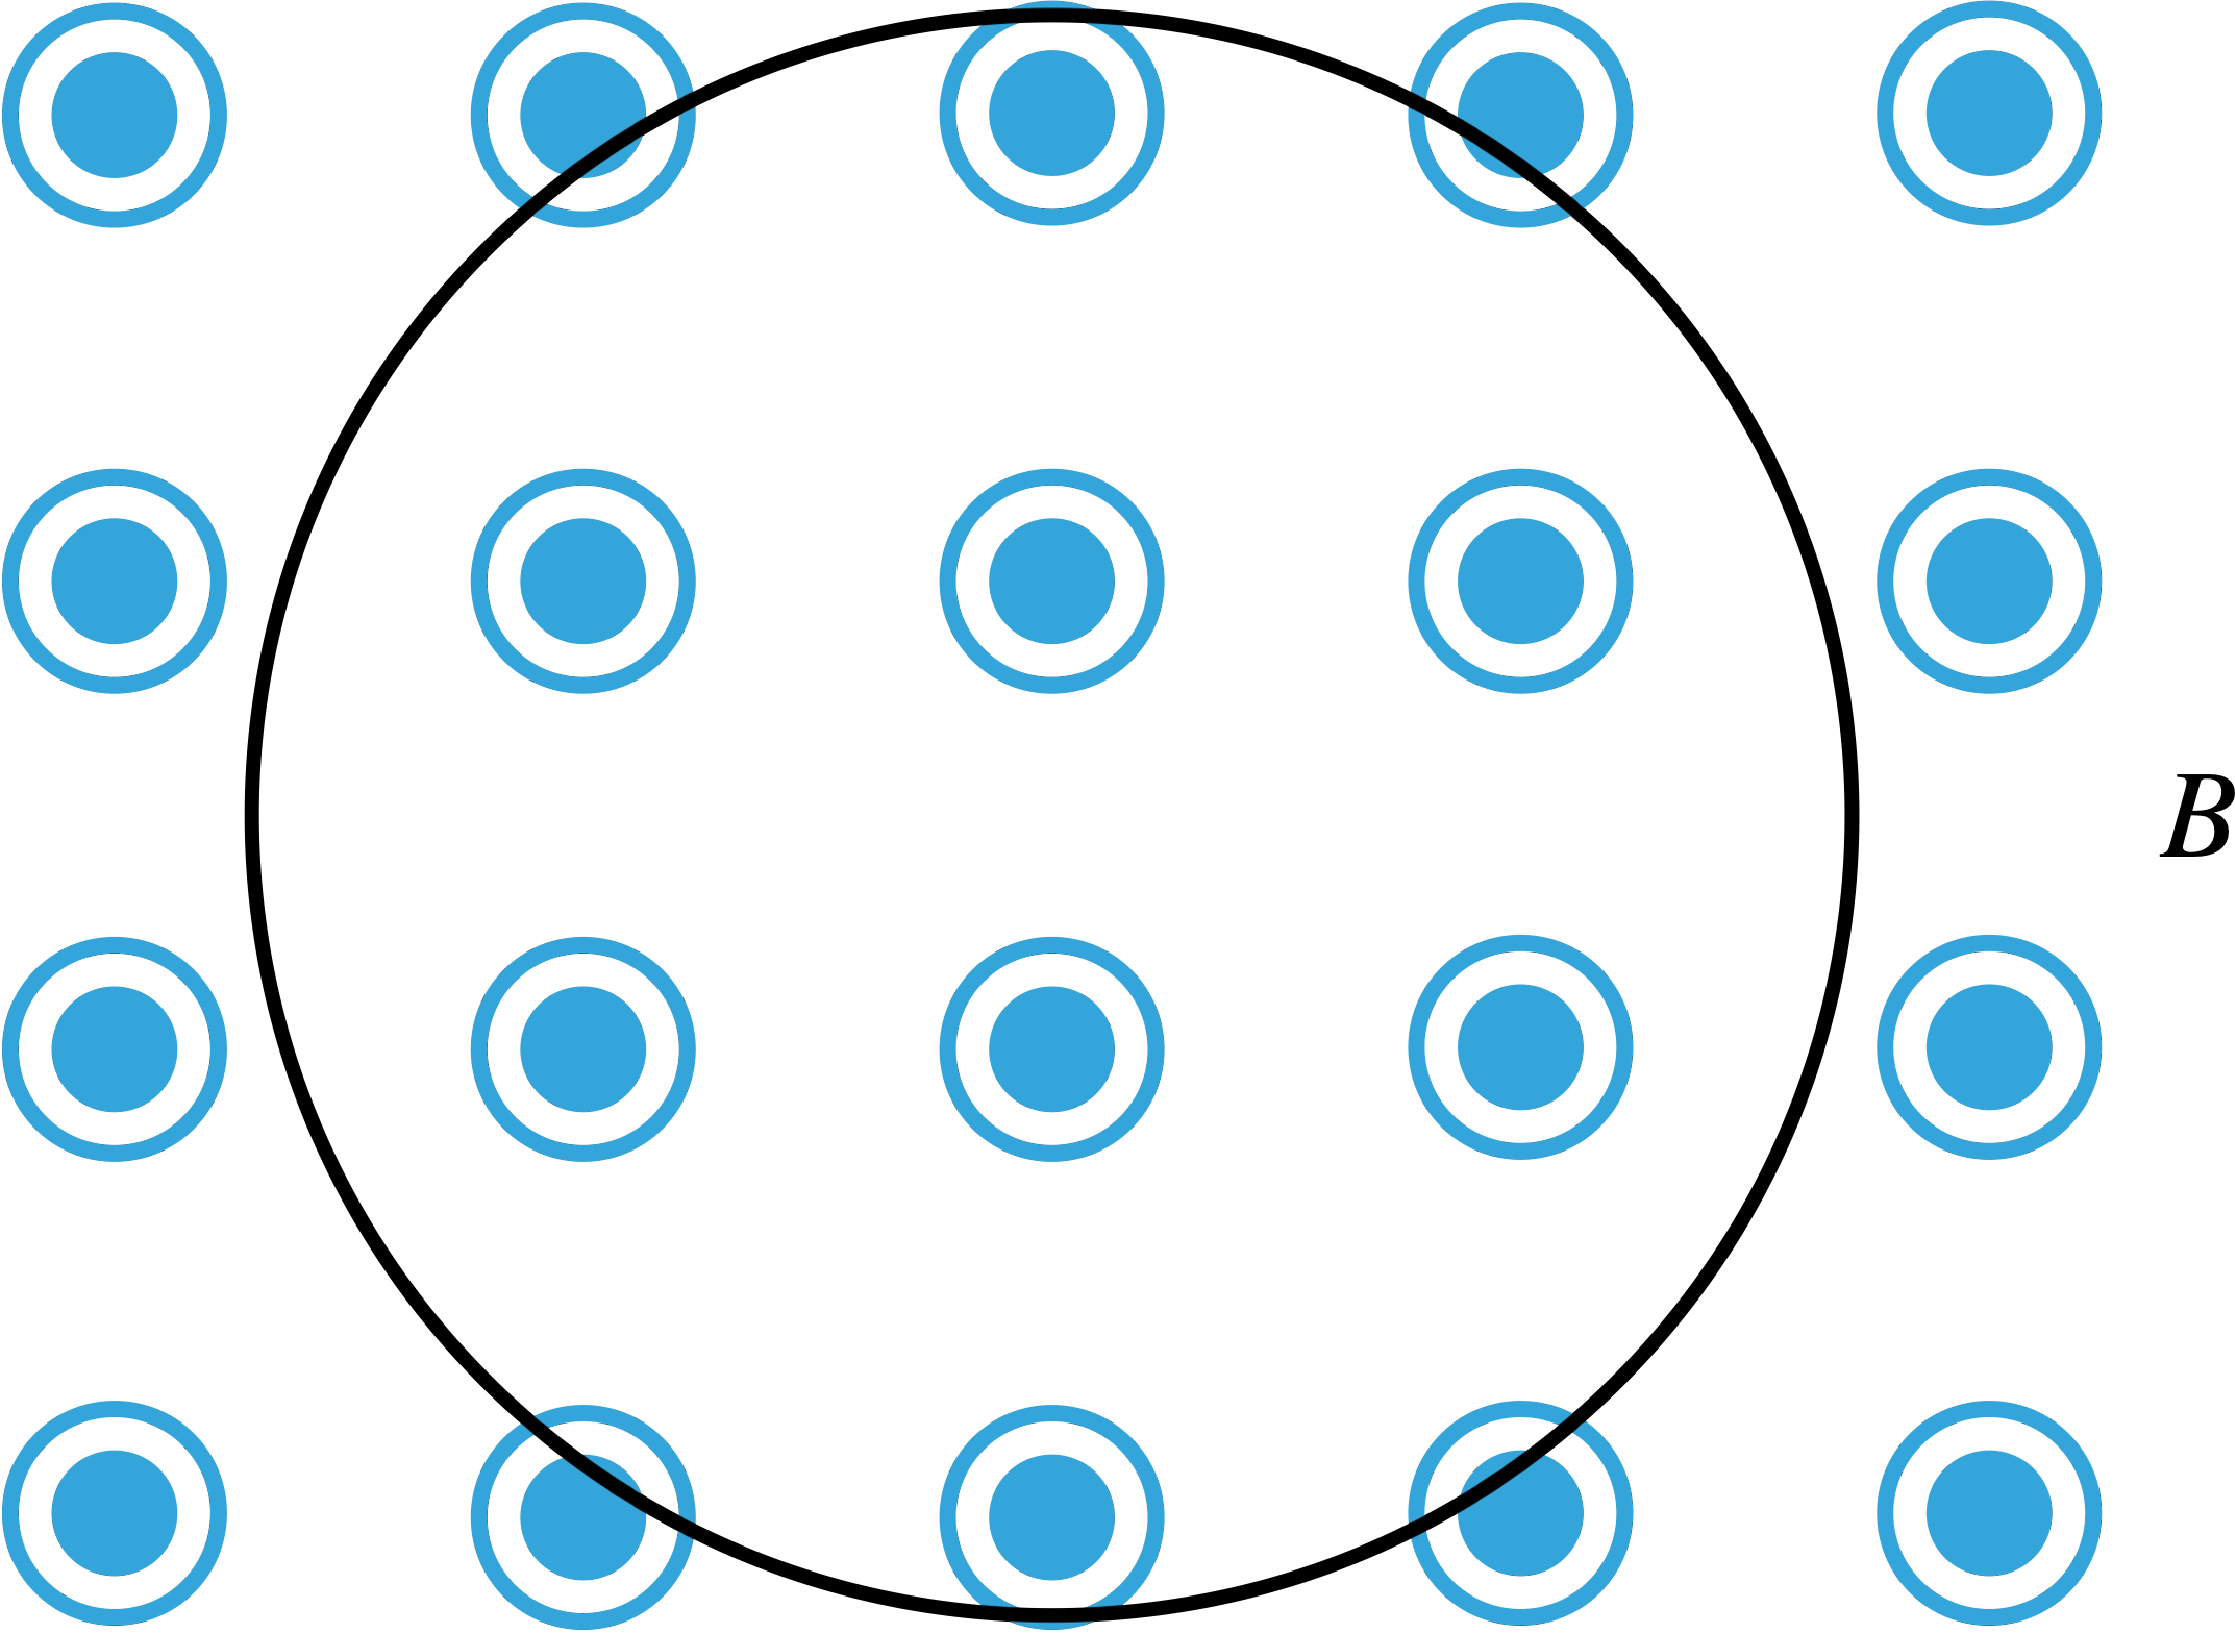
\includegraphics[width=.4\textwidth]{faraday.pdf}
\end{center}

\begin{parts}
	\part Initially (at time $t=0$) what is the magnitude of the induced emf in the loop?
	\vspace{3cm}
	\part What direction is the induced emf (what direction will induced current flow?)
\end{parts}